
% This LaTeX was auto-generated from an M-file by MATLAB.
% To make changes, update the M-file and republish this document.

\documentclass{article}
\usepackage{graphicx}
\usepackage{color}

\sloppy
\definecolor{lightgray}{gray}{0.5}
\setlength{\parindent}{10pt}
\usepackage[margin=1in]{geometry}

\begin{document}

\title{Dynamical Adaptation in ORNs}
\author{Srinivas Gorur-Shandilya}
\maketitle

    
    
\section*{Filter Estimation}

\begin{par}
How do we best calculate the filters? A summary of different ways of estimating the filters and results from each.
\end{par} \vspace{1em}

\subsection*{Contents}

\begin{itemize}
\setlength{\itemsep}{-1ex}
   \item Overview of different regularisation methods.
   \item Synthetic Data with No regularisation
   \item Synthetic Data: effect of regularisation
   \item Synthetic Data 2: effect of regularisation
   \item Real Data: effect of regularisation
\end{itemize}


\subsection*{Overview of different regularisation methods.}

\begin{par}
The filter \textit{K} is given by
\end{par} \vspace{1em}
\begin{par}
$$ \hat{C}*K=s'*f $$
\end{par} \vspace{1em}
\begin{par}
where $\hat{C}$ is the regularised covariance matrix \textit{C}, \textit{s} is a \textit{N} x \textit{M} matrix of the time-shifted stimulus and \textit{f} is the response vector. \textit{N} is the filter length, and \textit{M} is the length of the stimulus and response vectors - \textit{N}.
\end{par} \vspace{1em}
\begin{par}
\textit{C} is the unscaled covariance matrix and is given by:
\end{par} \vspace{1em}
\begin{par}
$$ C=s^{T}*s $$
\end{par} \vspace{1em}
\begin{par}
can be regularised by different means:
\end{par} \vspace{1em}
\begin{par}
1) Carlotta regularises \textit{C} using:
\end{par} \vspace{1em}
\begin{par}
$$ \hat{C}=C+\hat{r}I $$
\end{par} \vspace{1em}
\begin{par}
2) and Damon suggested:
\end{par} \vspace{1em}
\begin{par}
$$ \hat{C}=\frac{(C+\hat{r}I)*\mathrm{tr}(C)}{(\mathrm{tr}(C)+\hat{r}N)} $$
\end{par} \vspace{1em}
\begin{par}
where \textit{I} is the identity matrix and \textit{r} is a free parameter called the regularisation factor that suppresses the high-frequency components of \textit{K}. $\hat{r}$  is obtained by scaling \textit{r} by $\mu$,  the mean of the Eigenvalues of the covariance matrix \textit{C}. \textit{s} is the stimulus vector (e.g. the PID) and \textit{f} is the response vector (here, the firing rate of the ORN). In practice, \textit{K} is estimated by a left matrix division:
\end{par} \vspace{1em}
\begin{par}
$$ K=C\setminus(s'*f) $$
\end{par} \vspace{1em}


\subsection*{Synthetic Data with No regularisation}

\begin{par}
Synthetic data is prepared using Gaussian random inputs and an exponential filter, and the output is the convolution of the input with the exponential filter, with 10\% noise.
\end{par} \vspace{1em}
\begin{par}
The following figure shows filters estimated using the three methods shown above, with zero regularisation. The actual filter is in black, and each method is coloured differently.
\end{par} \vspace{1em}

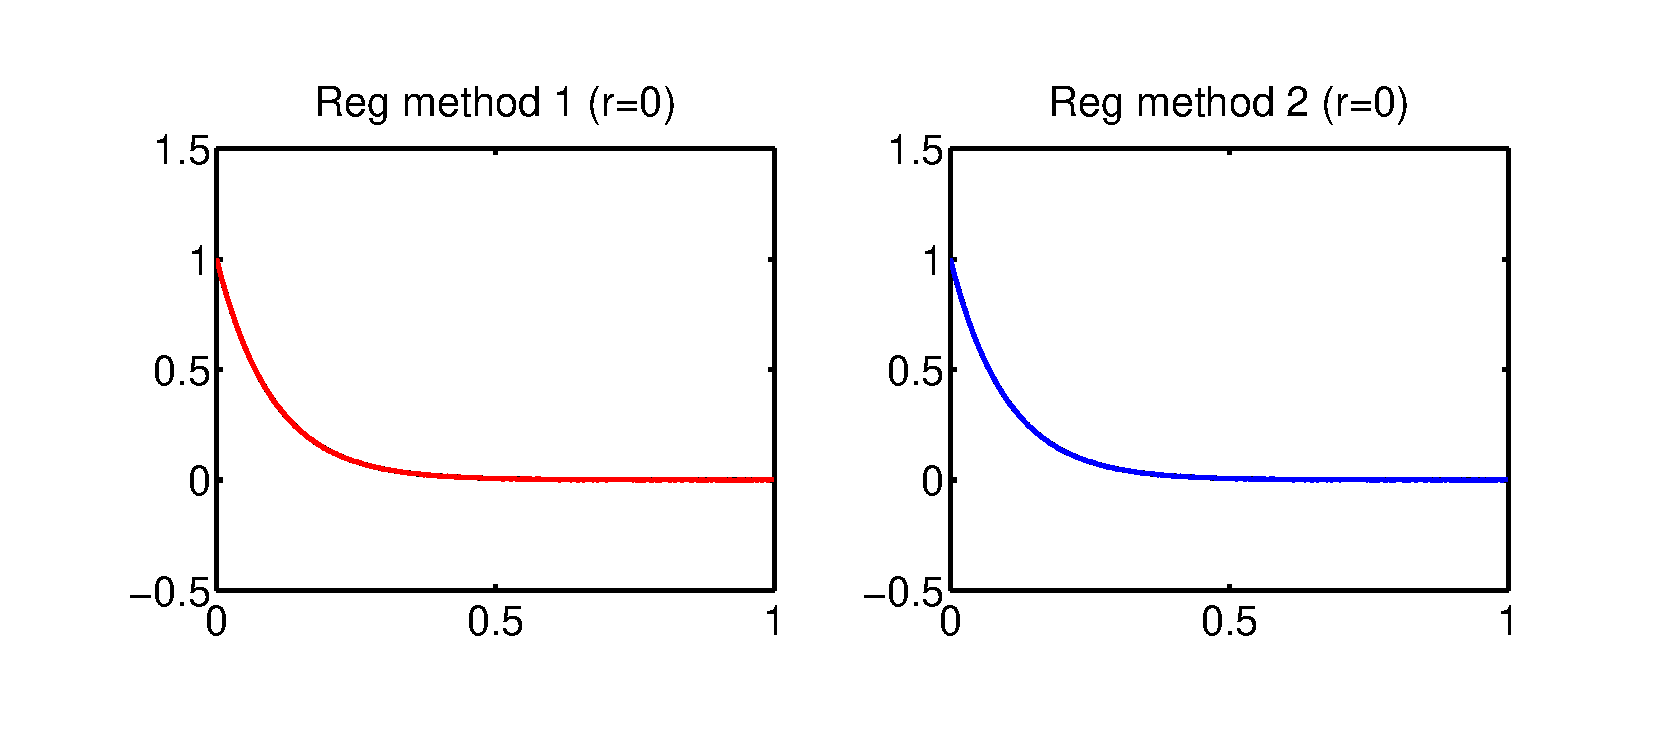
\includegraphics [width=\textwidth]{FilterEstimation_01.pdf}


\subsection*{Synthetic Data: effect of regularisation}

\begin{par}
what is the effect of increasing \textit{r}, the regularisation parameter on each of these methods? Here we systematically vary \textit{r}, and pick the best filter that minimises
\end{par} \vspace{1em}
\begin{par}
$$ \arg\min_{r}\left\Vert \frac{e(r)-1}{1},\frac{S(r)-\min(S)}{\min(S)},\frac{\left|m(r)-1\right|}{1}\right\Vert _{\infty} $$
\end{par} \vspace{1em}
\begin{par}
where \textit{e} is the coefficient of determination (r-square) of the prediction w.r.t to the actual data, \textit{S} is the sum of absolute values of the derivative of the filter \textit{K}, and \textit{m} is the slope of the best fit of the prediction to the data. Minimising (\textit{e} - 1) minimises the error of the fit. Minimising \textit{S} minimises the high-frequency components in the filter, and prevents over-fitting. We also want the slope \textit{m} to be as close to 1 as possible. If \textit{S} has a minimum, that value of \textit{r} is automatically chosen.
\end{par} \vspace{1em}
\begin{par}
In each of the plots below, the variation of error, filter sum, filter height, gain, and condition number of \textit{C} is show with \textit{r}, the regularisation factor, in units of $\mu$. The error is calculated from the prediction to the actual output. The filter sum is the sum of the absolute values of the filter. Very high values here indicate the filter dominated by high-frequency components. The filter height is the peak of the filter. The gain is the slope of the best fit line of the data to the prediction. The condition number is the ratio of the largest to the smallest eigenvalue of \textit{C}. Values of the condition number close to 1 mean that the matrix is easier to invert.  The figure below shows how varying \textit{r} affects reg method 1:
\end{par} \vspace{1em}

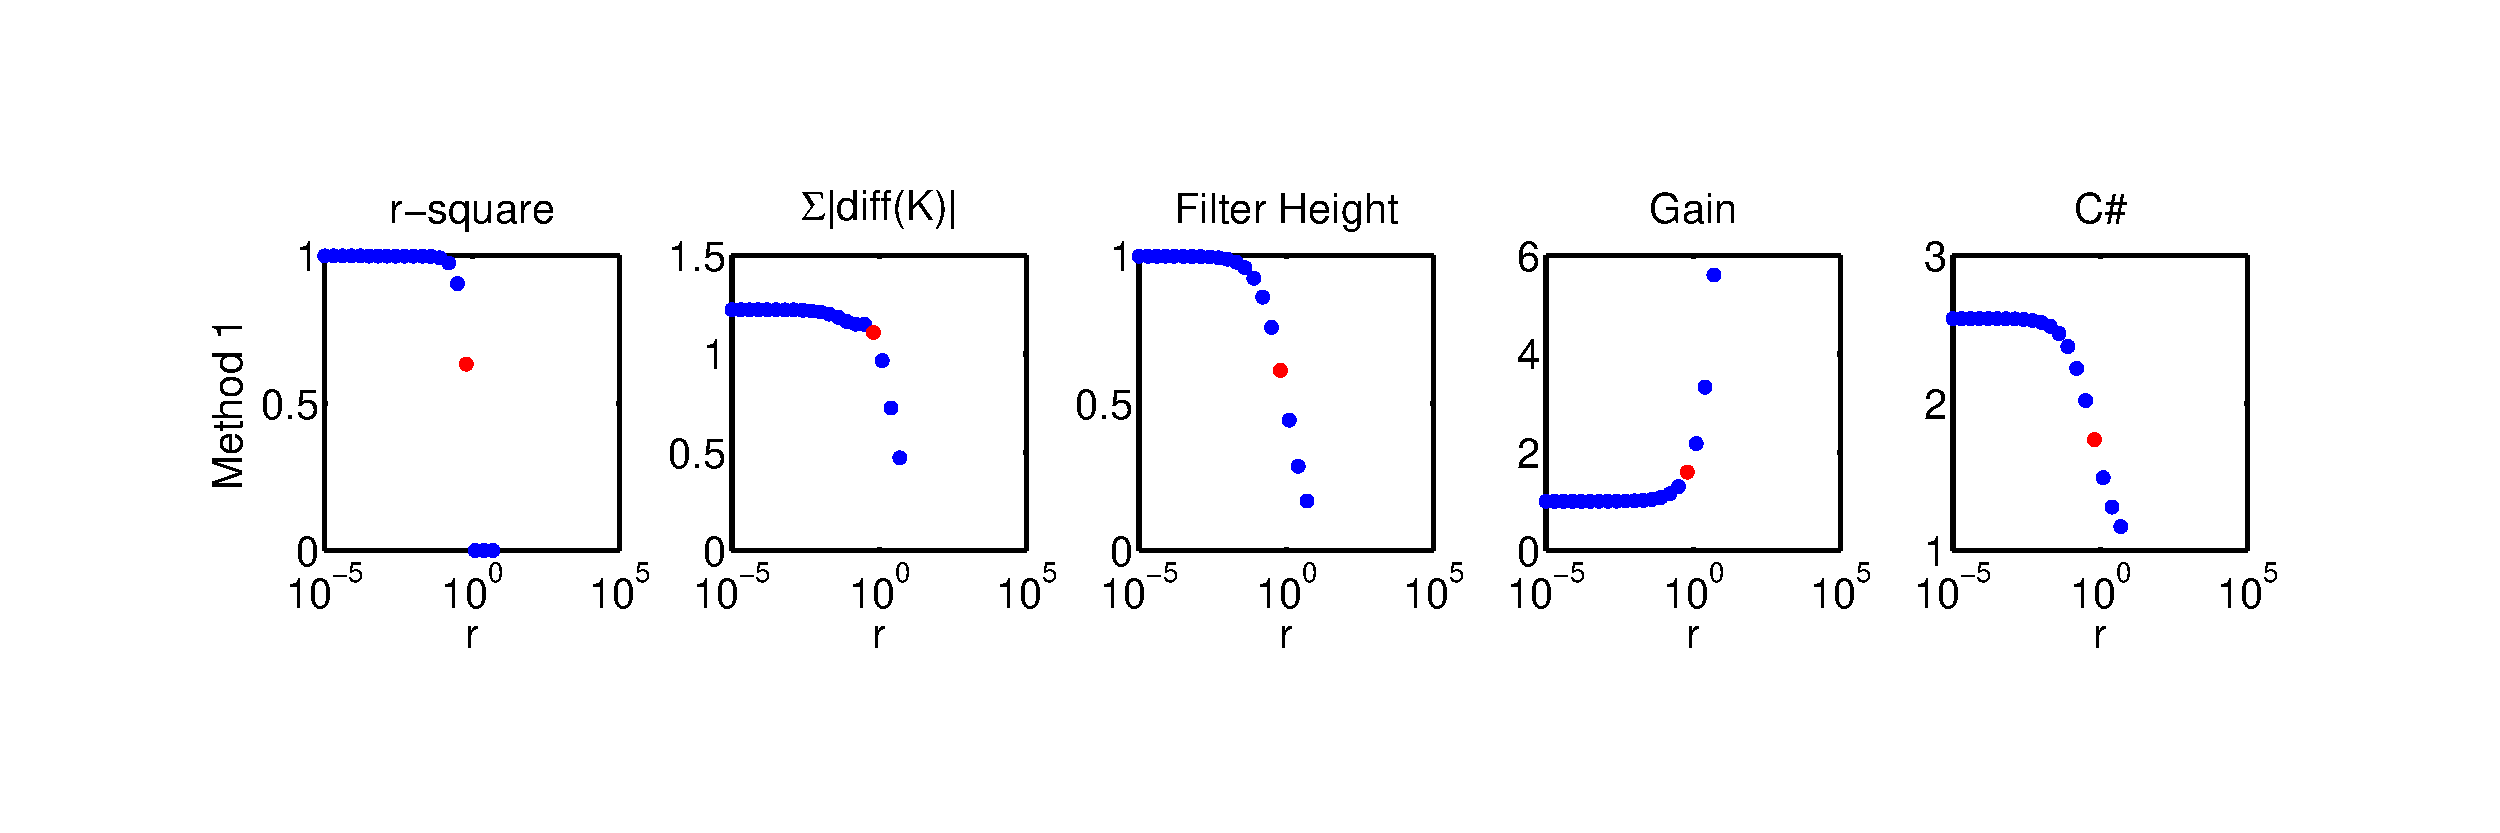
\includegraphics [width=\textwidth]{FilterEstimation_02.pdf}
\begin{par}
the figure below shows how varying \textit{r} affects reg method 2:
\end{par} \vspace{1em}

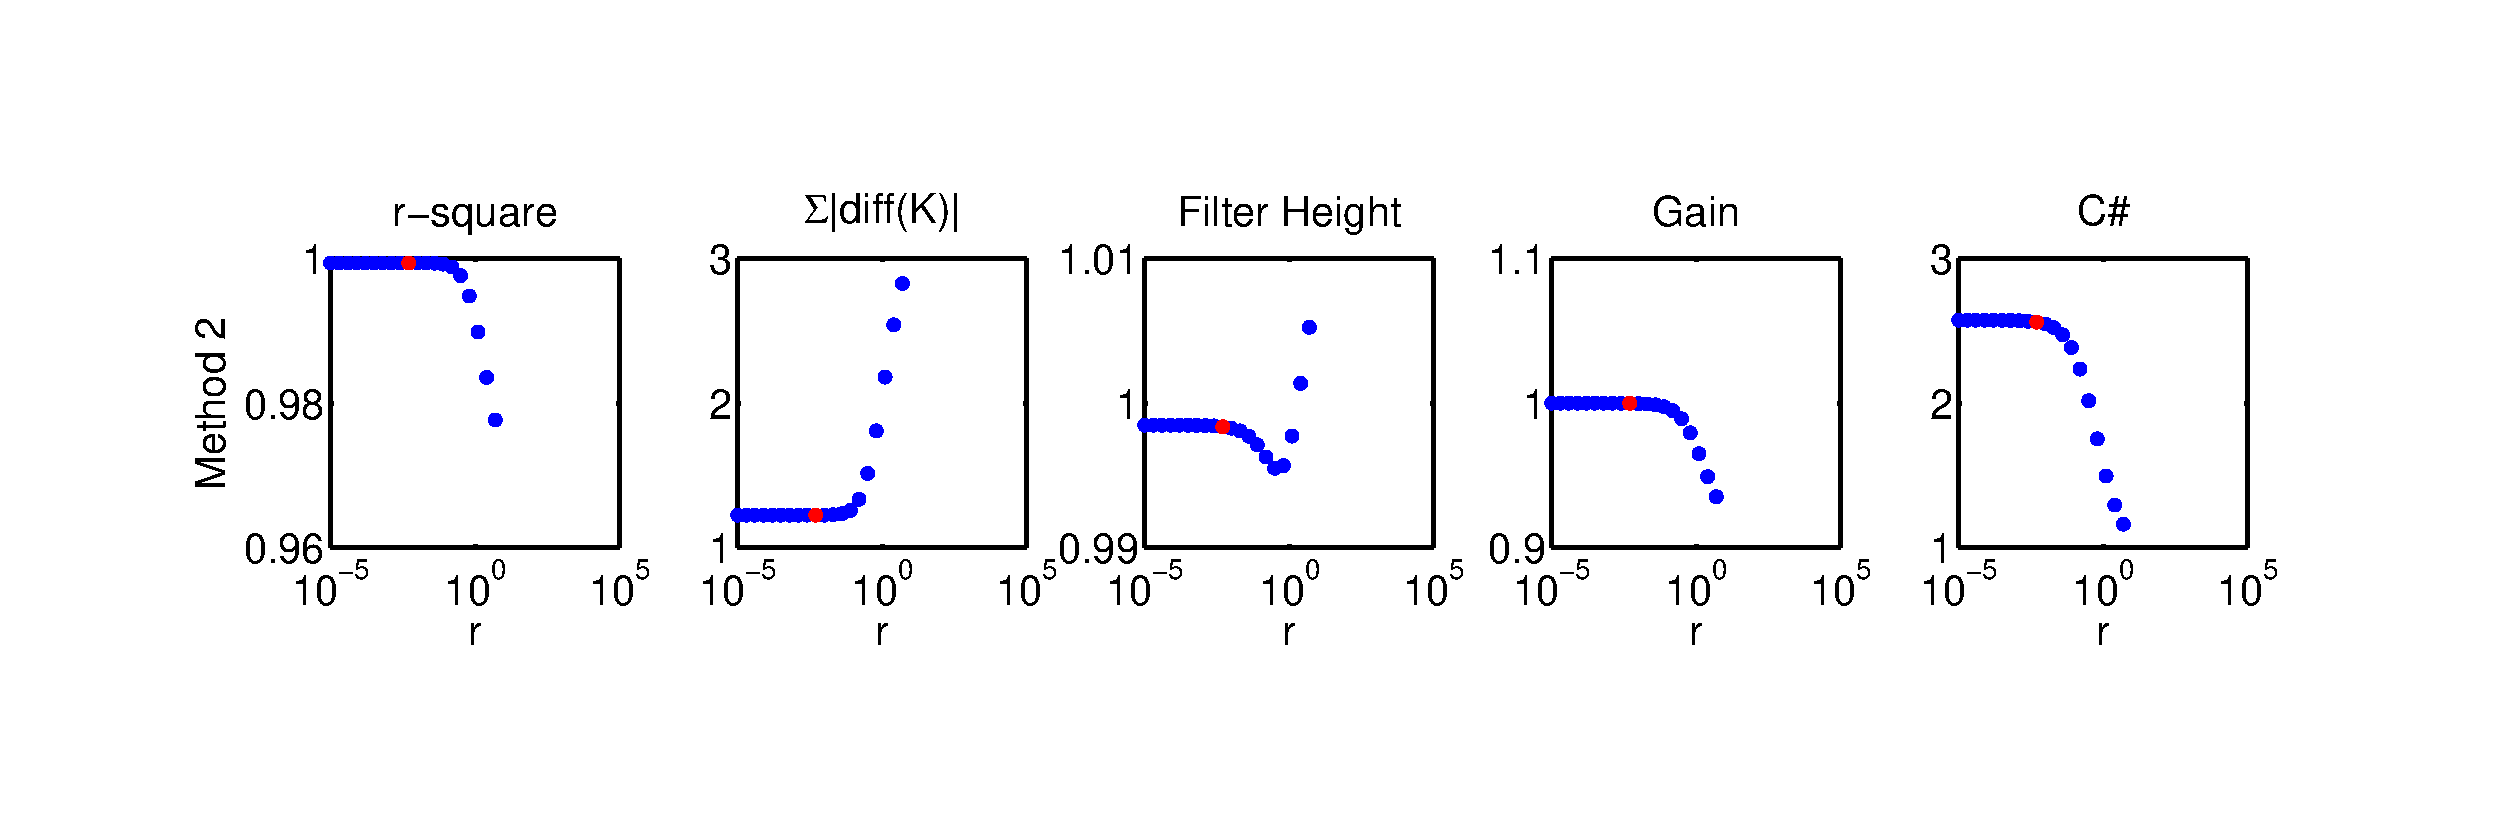
\includegraphics [width=\textwidth]{FilterEstimation_03.pdf}
\begin{par}
The best filters are shown below for the two reg. methods:
\end{par} \vspace{1em}

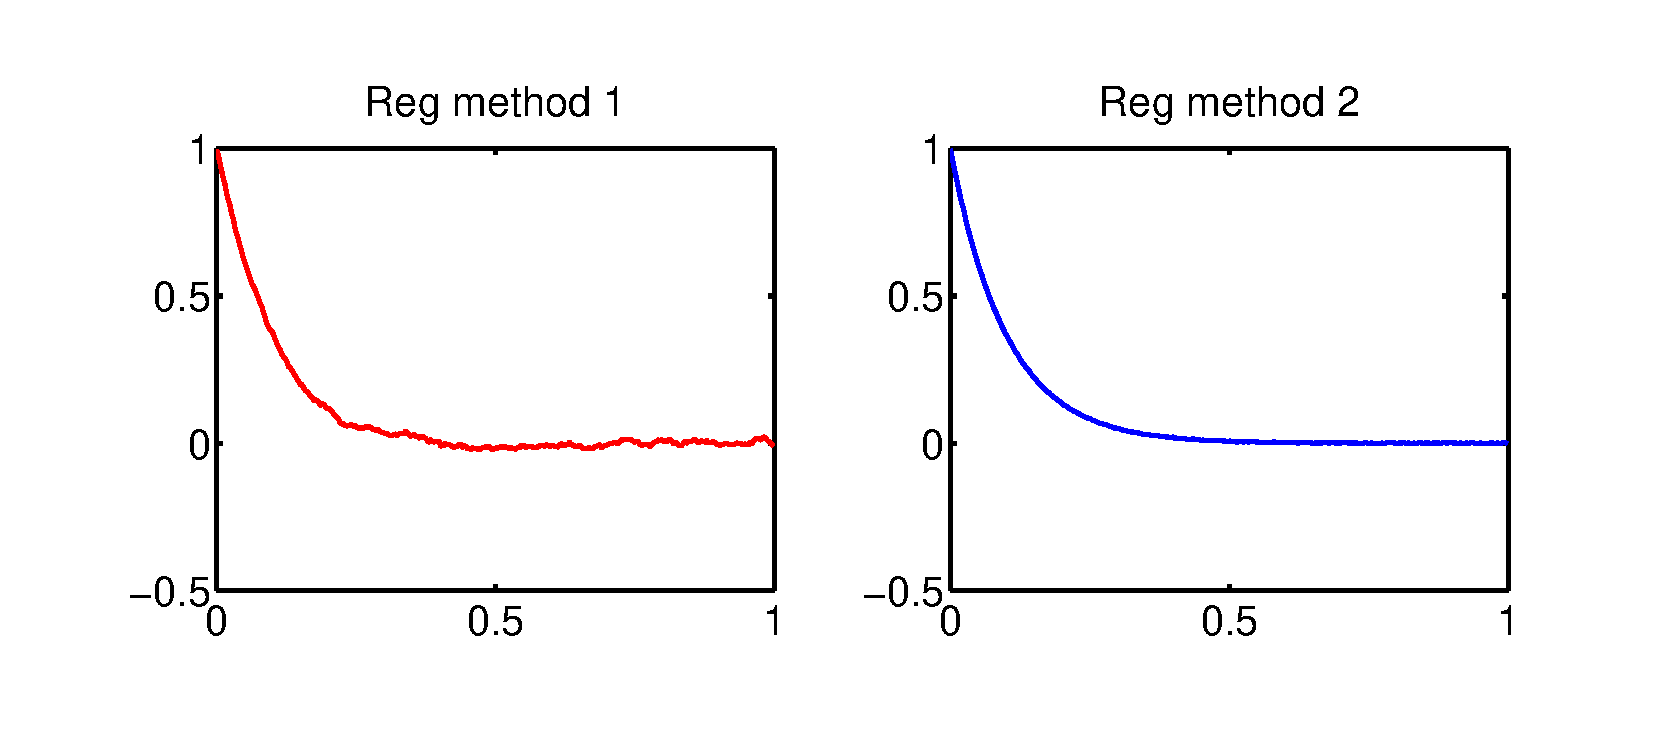
\includegraphics [width=\textwidth]{FilterEstimation_04.pdf}


\subsection*{Synthetic Data 2: effect of regularisation}

\begin{par}
We now create a new synthetic dataset, identical to the old one, except we filter the white noise input with some boxcar filter to remove high frequency components from the input. We find the best filters as before, and look at how regularisation parameter affects the choice of filter.
\end{par} \vspace{1em}
\begin{par}
The best filters are shown below for the two reg. methods:
\end{par} \vspace{1em}

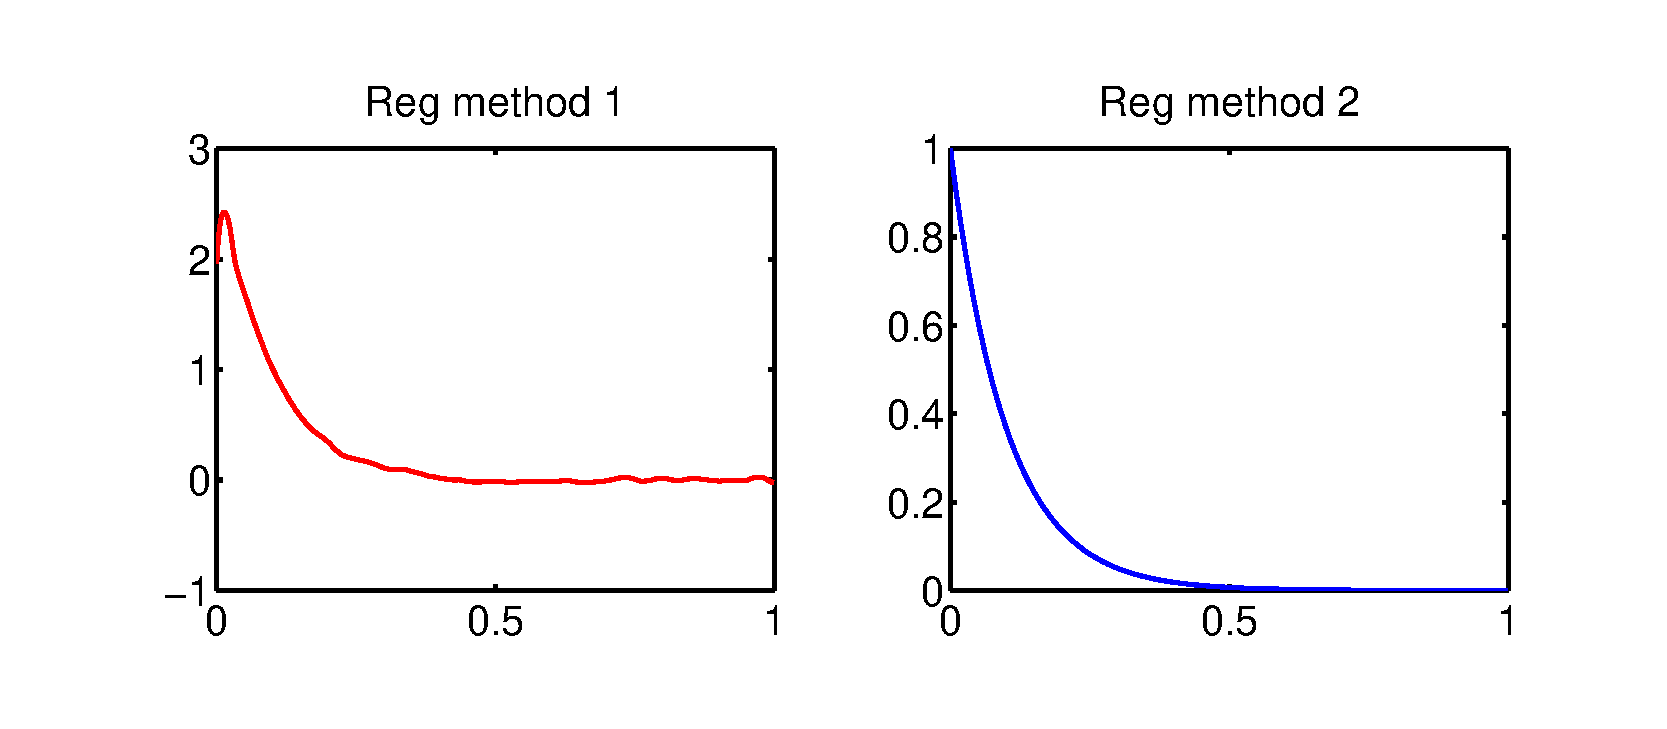
\includegraphics [width=\textwidth]{FilterEstimation_05.pdf}
\begin{par}
the figure below shows how varying \textit{r} affects reg method 1:
\end{par} \vspace{1em}

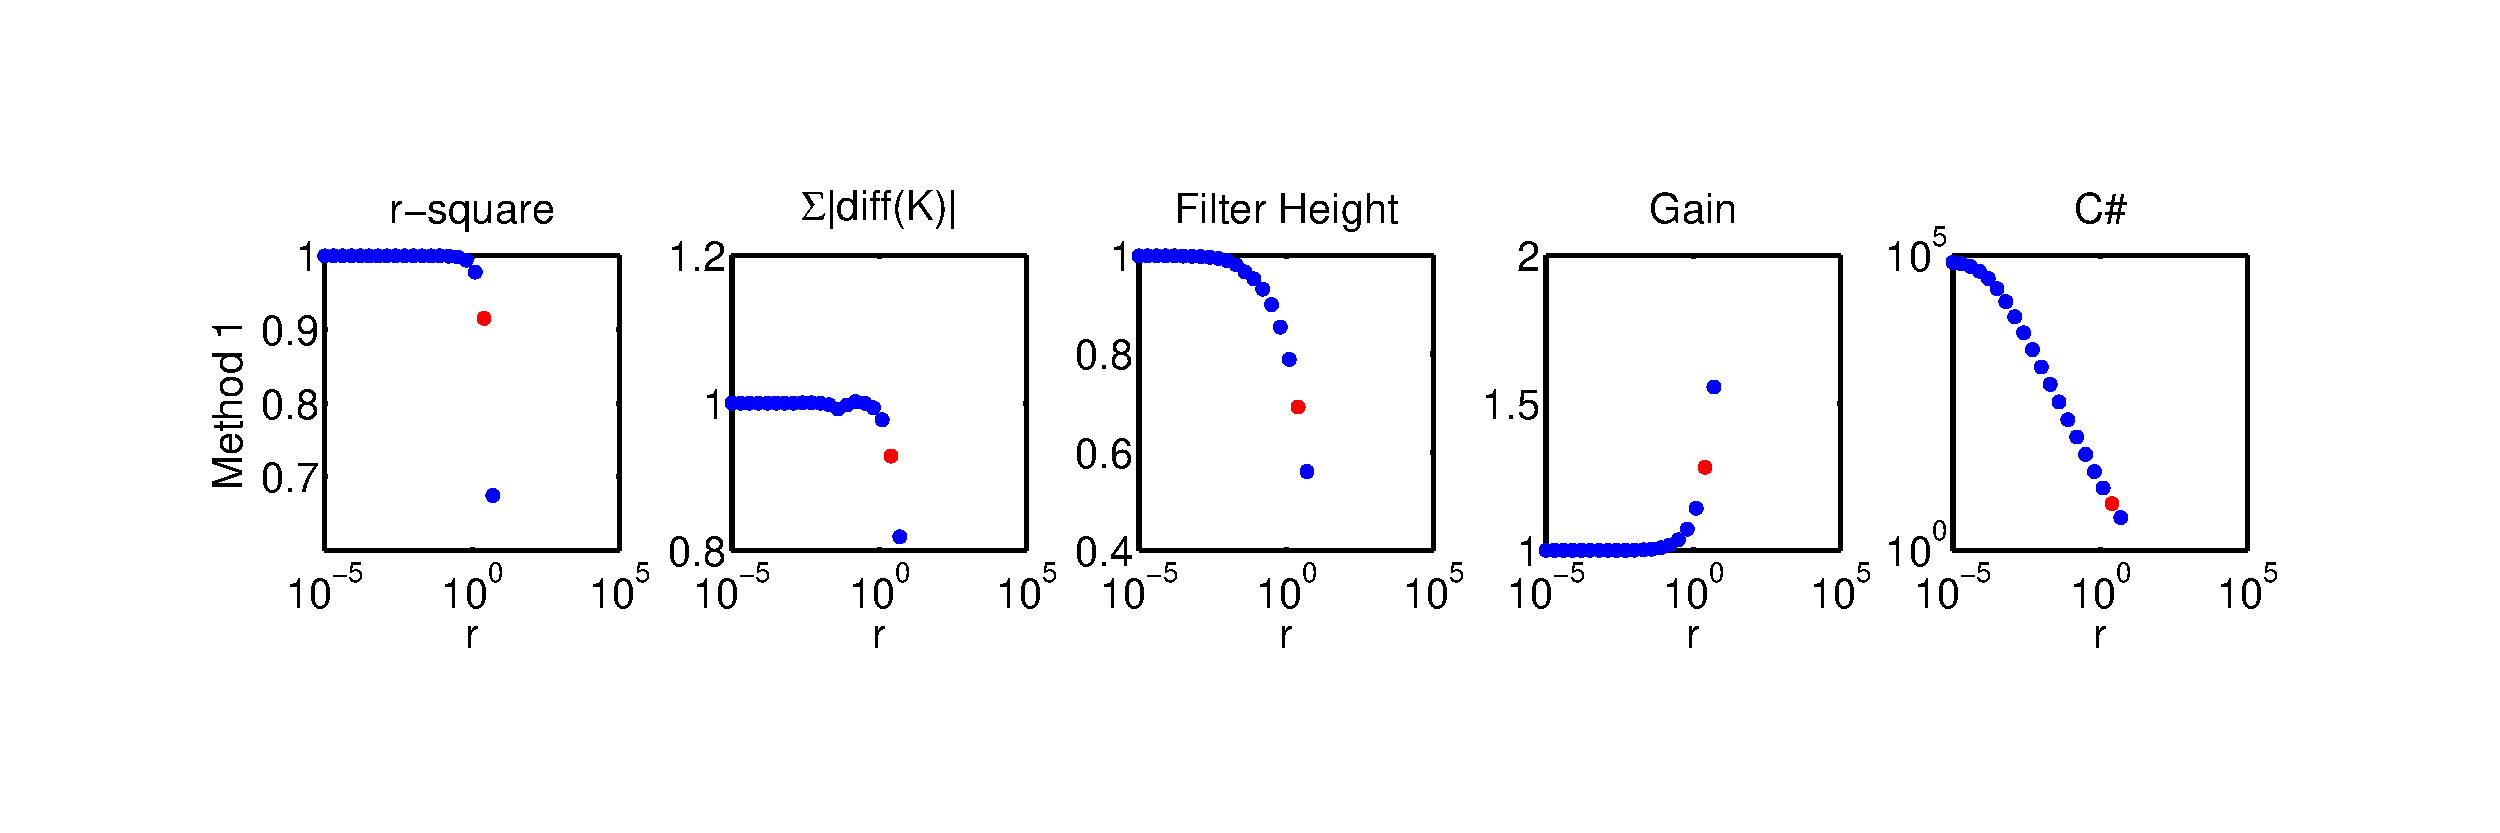
\includegraphics [width=\textwidth]{FilterEstimation_06.pdf}
\begin{par}
the figure below shows how varying \textit{r} affects reg method 2:
\end{par} \vspace{1em}

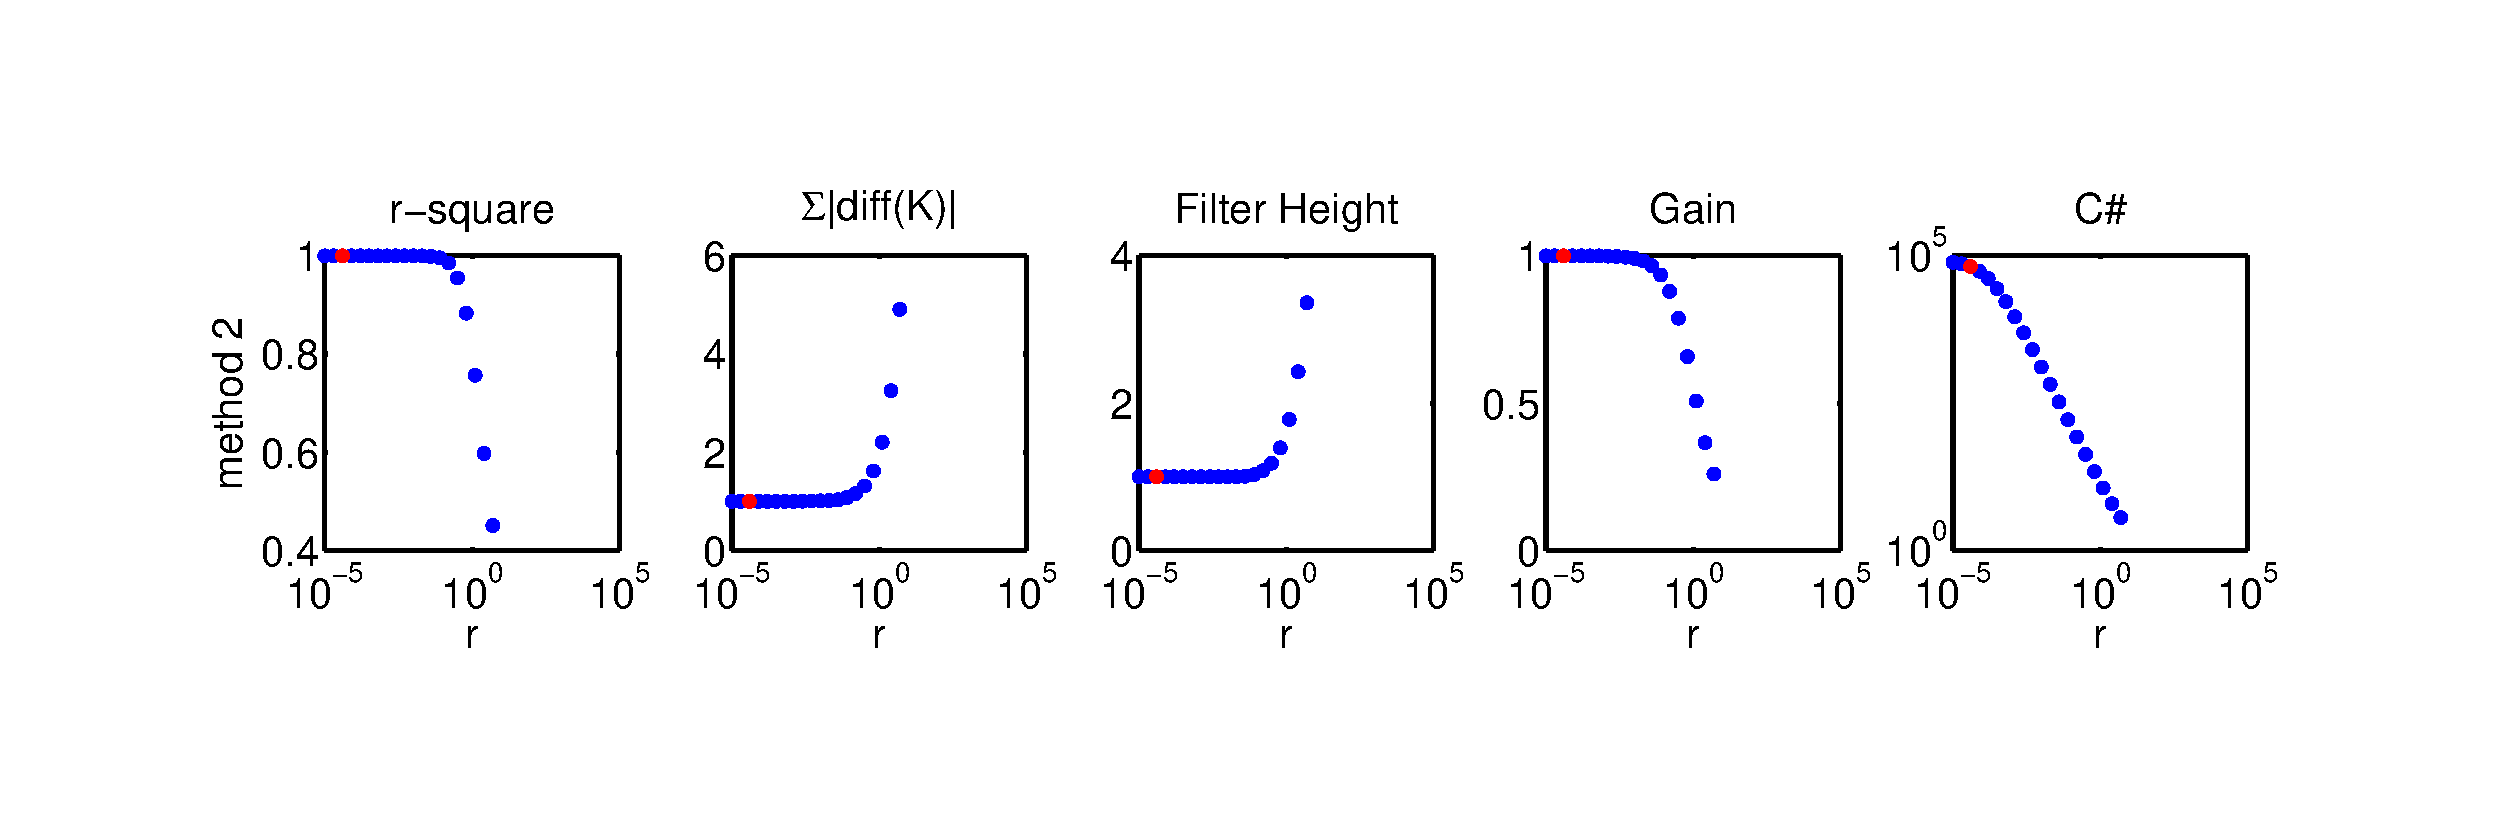
\includegraphics [width=\textwidth]{FilterEstimation_07.pdf}


\subsection*{Real Data: effect of regularisation}

\begin{par}
We use PID traces as the input, and the firing rate of a ORN as the output. The data looks like this:
\end{par} \vspace{1em}

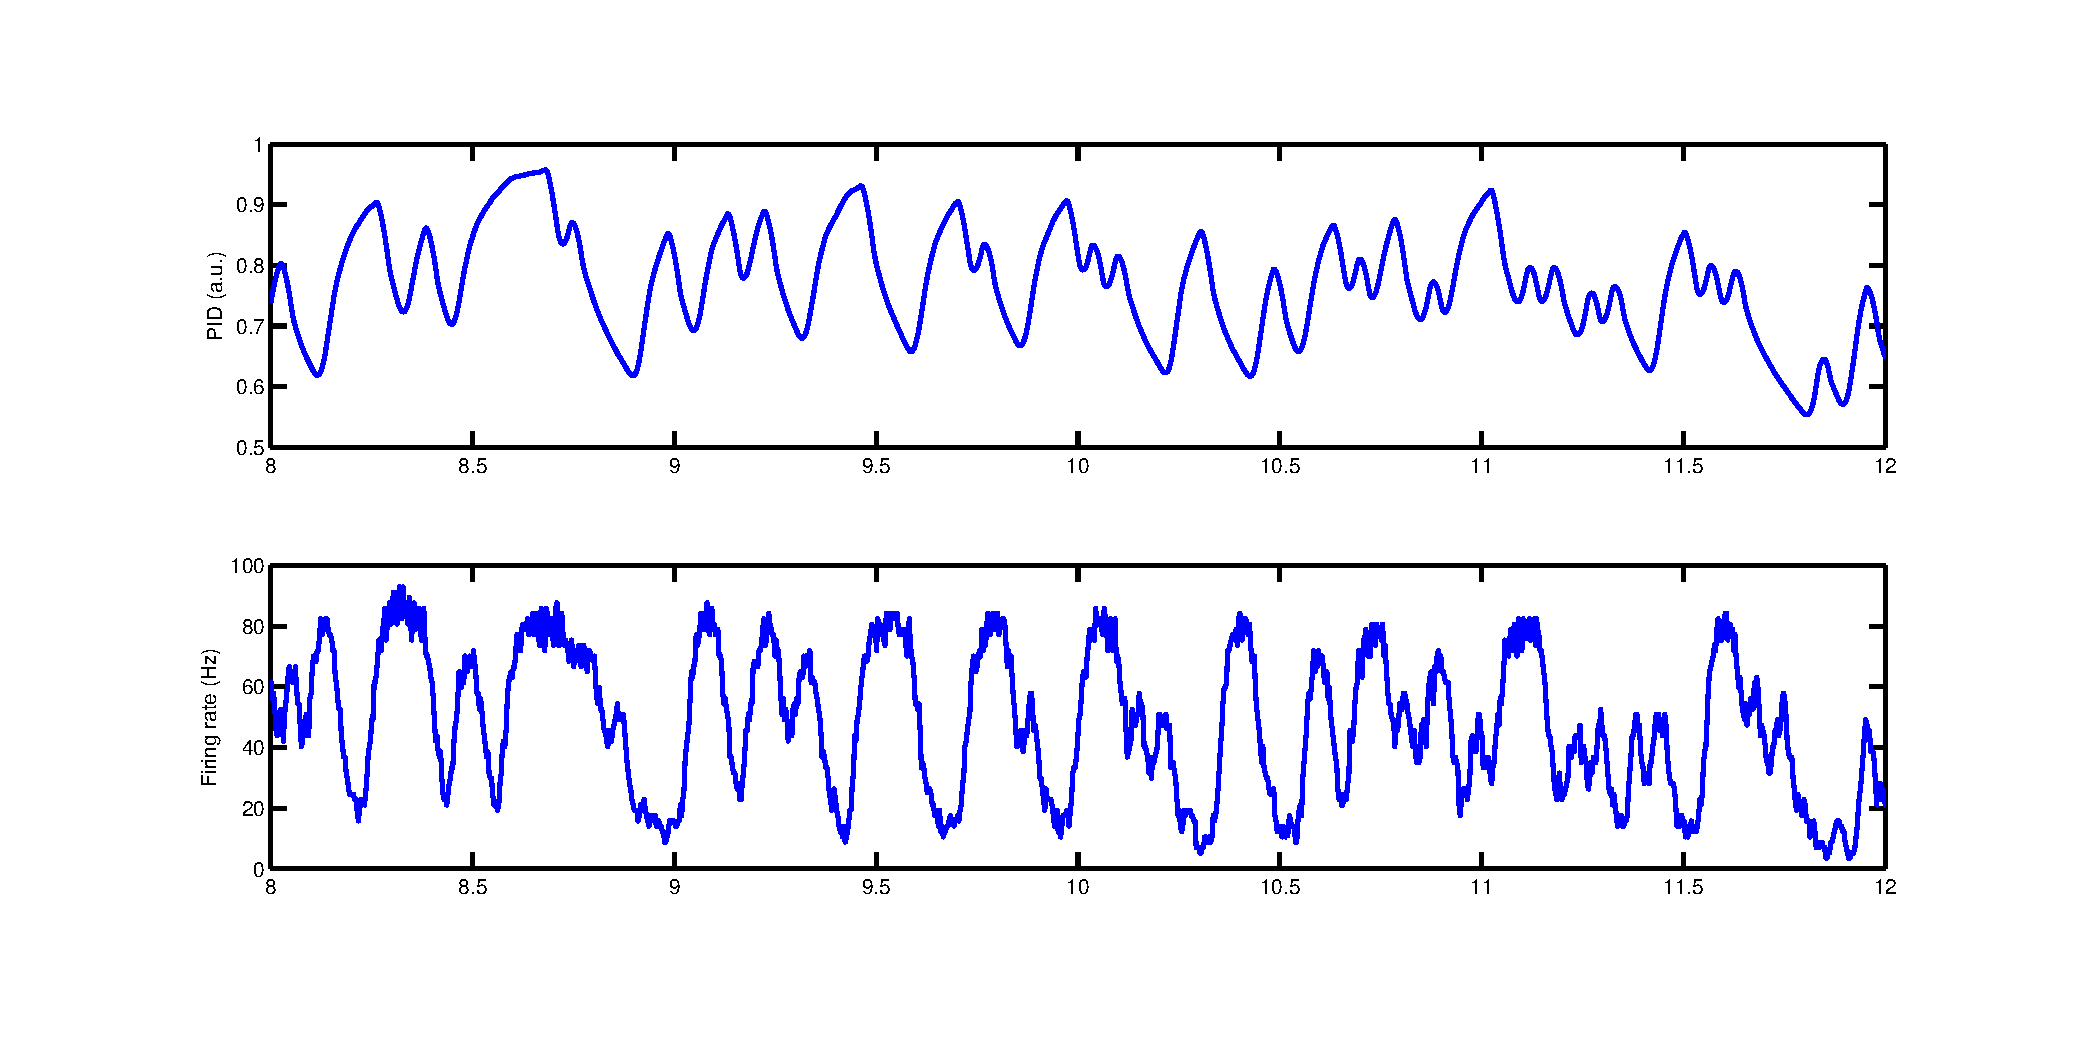
\includegraphics [width=\textwidth]{FilterEstimation_08.pdf}
\begin{par}
The covariance of the input matrix \textit{C} looks like:
\end{par} \vspace{1em}

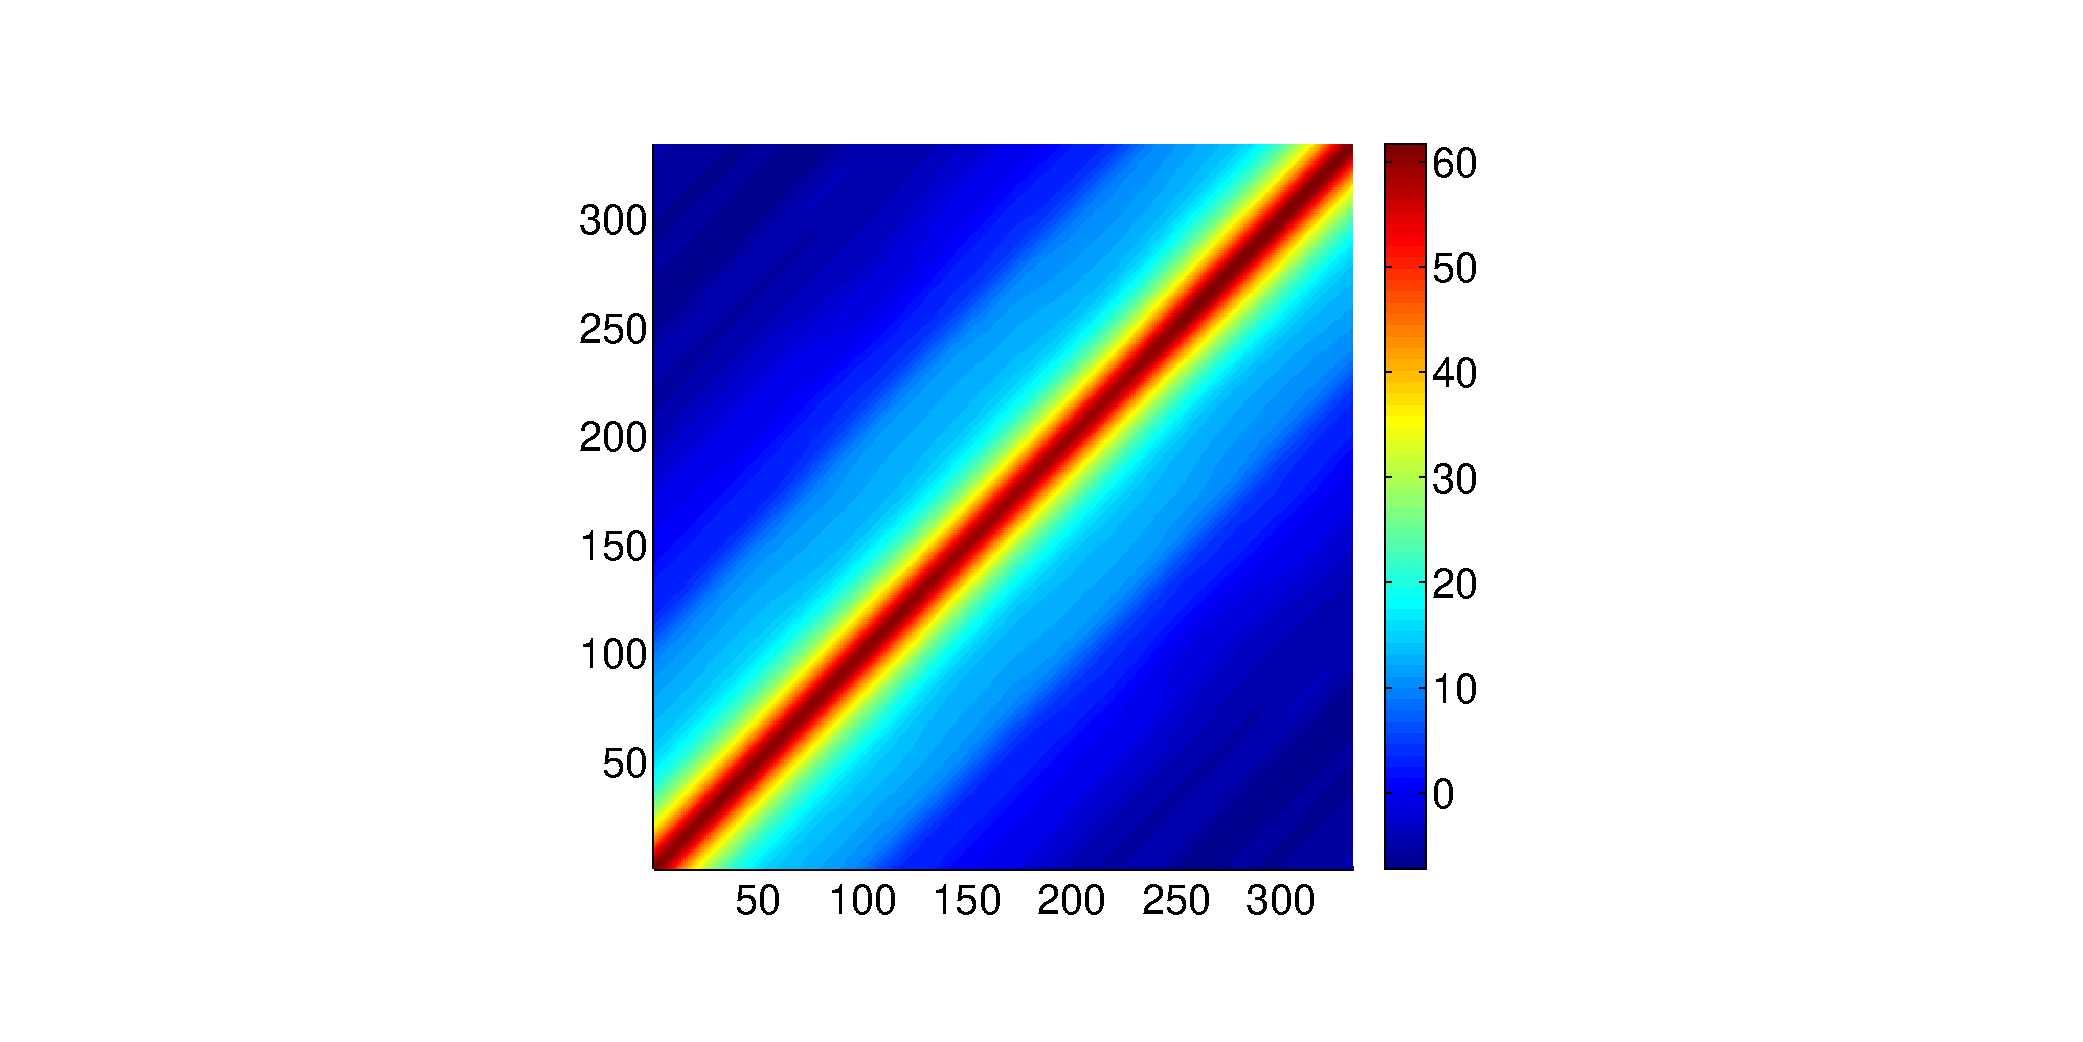
\includegraphics [width=\textwidth]{FilterEstimation_09.pdf}
\begin{par}
Regularisation adds a large diagonal matrix to this, in effect making it look more like a diagonal matrix. Here, the mean of the eigenvalues of \textit{C} has been added to the diagonal. This is essentially what Method 1 does.
\end{par} \vspace{1em}

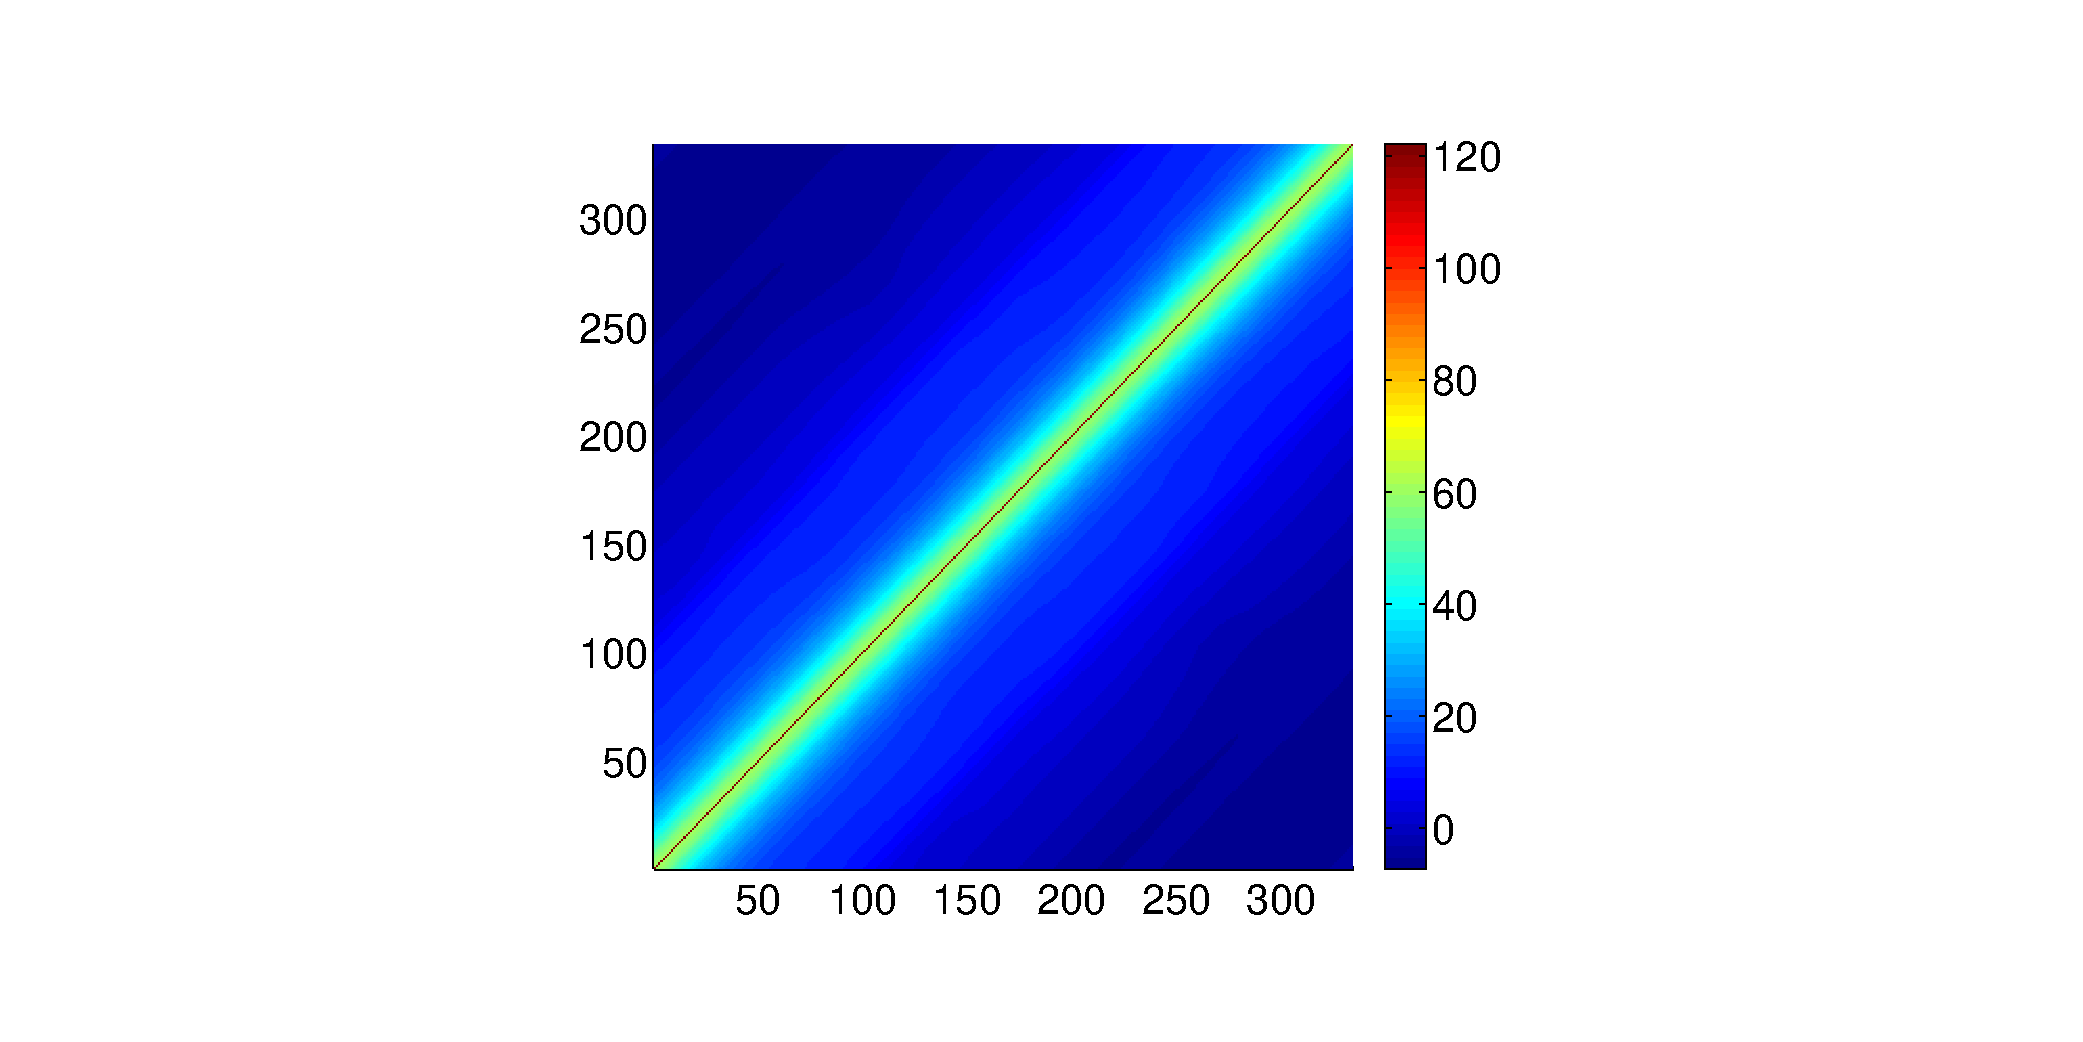
\includegraphics [width=\textwidth]{FilterEstimation_10.pdf}
\begin{par}
The effect of regularisation using method 2 is shown on the correlation matrix below. The same \textit{r} is used, i.e., the mean of the eigenvalues of \textit{C}.
\end{par} \vspace{1em}

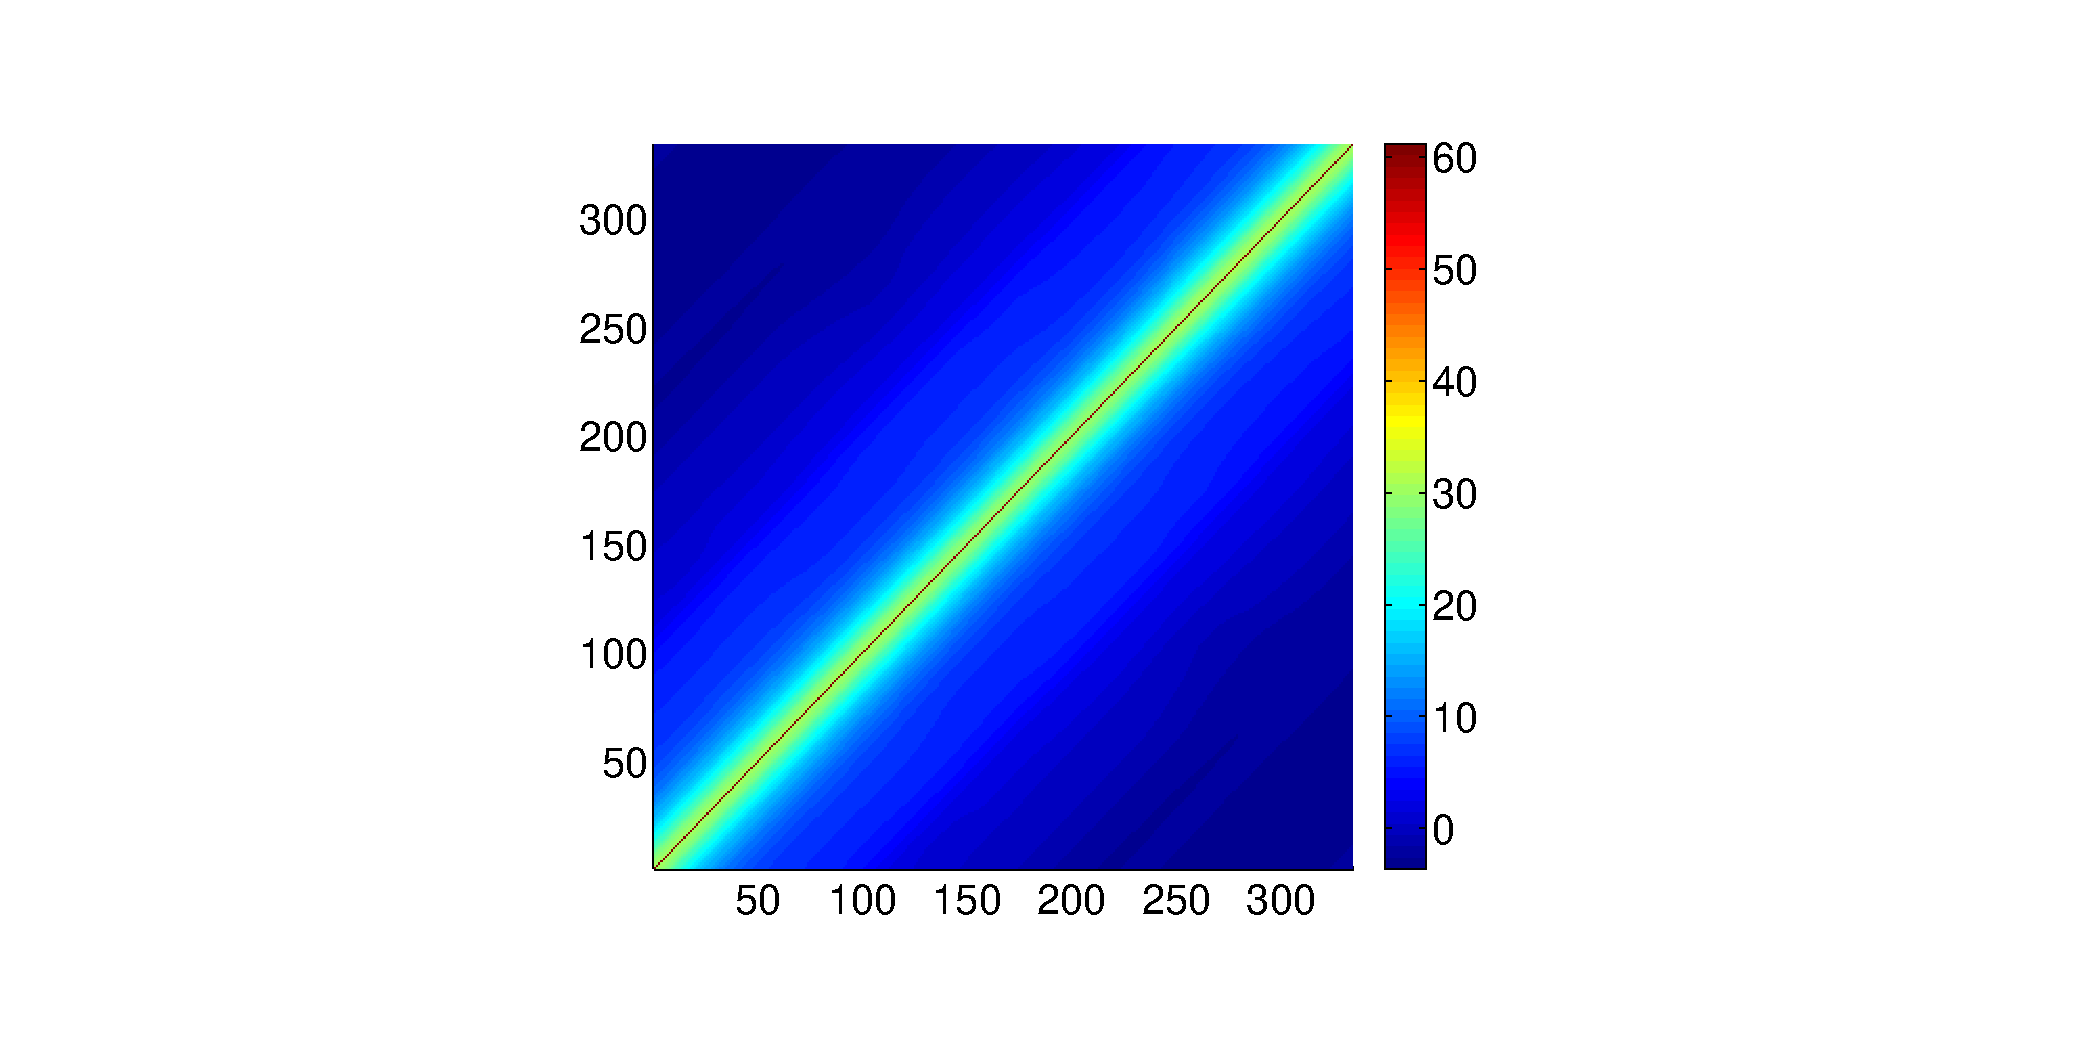
\includegraphics [width=\textwidth]{FilterEstimation_11.pdf}
\begin{par}
Once again, we repeat the filter extraction.
\end{par} \vspace{1em}
\begin{par}
the figure below shows how varying \textit{r} affects reg method 1:
\end{par} \vspace{1em}

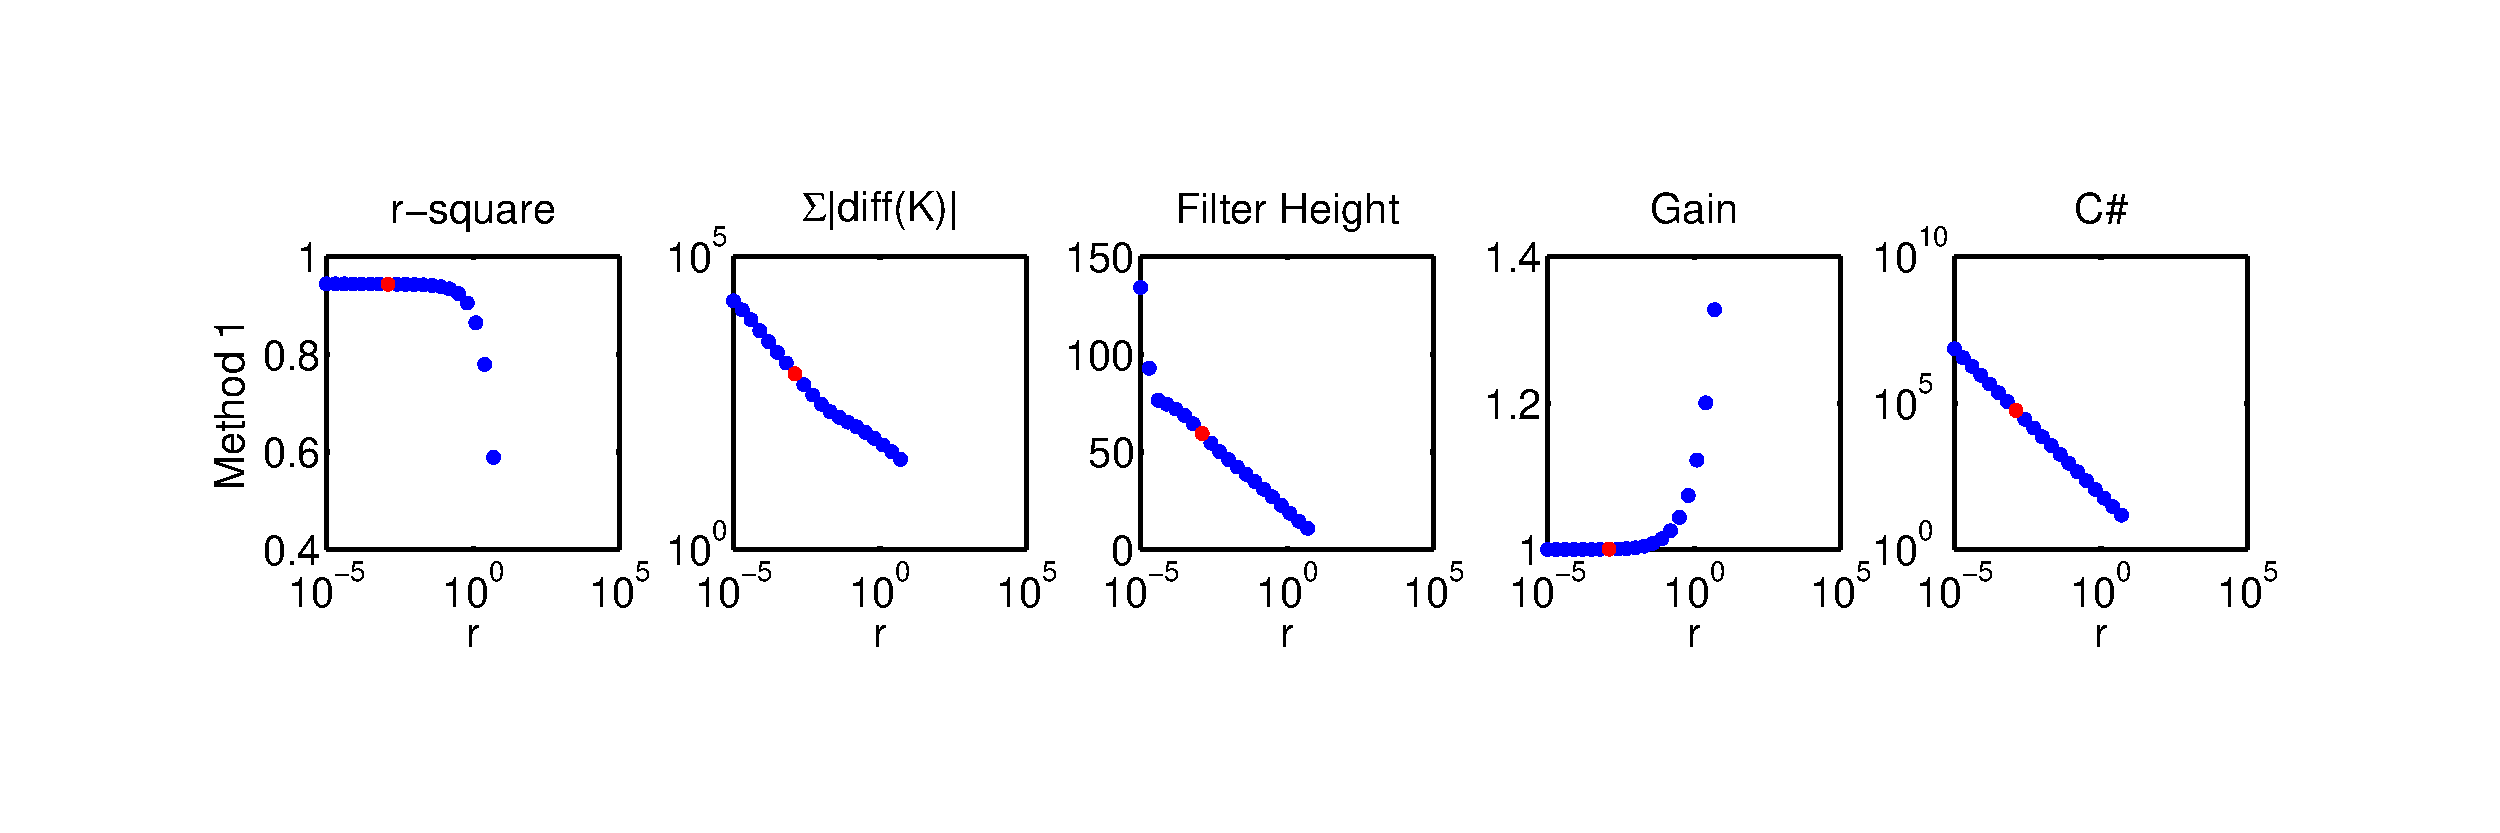
\includegraphics [width=\textwidth]{FilterEstimation_12.pdf}
\begin{par}
the figure below shows how varying \textit{r} affects reg method 2:
\end{par} \vspace{1em}

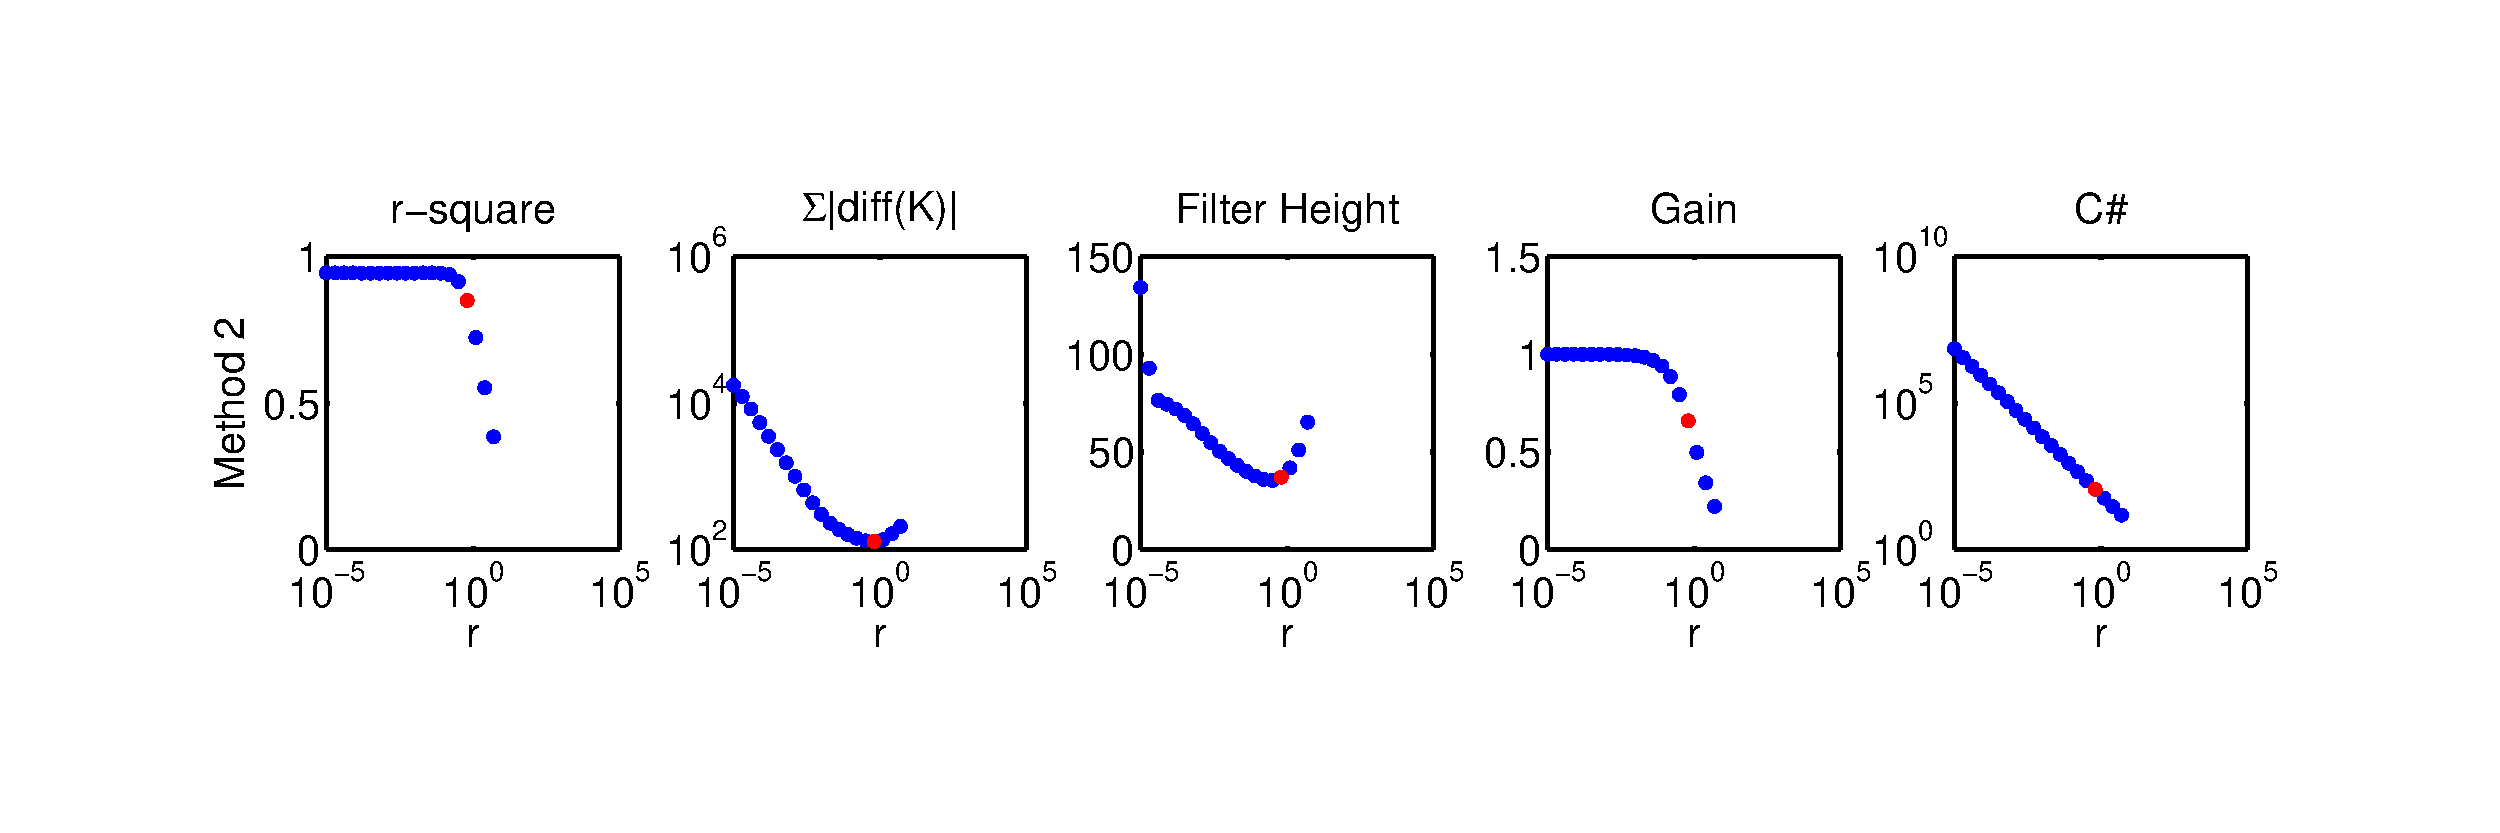
\includegraphics [width=\textwidth]{FilterEstimation_13.pdf}
\begin{par}
and the best filters look like:
\end{par} \vspace{1em}

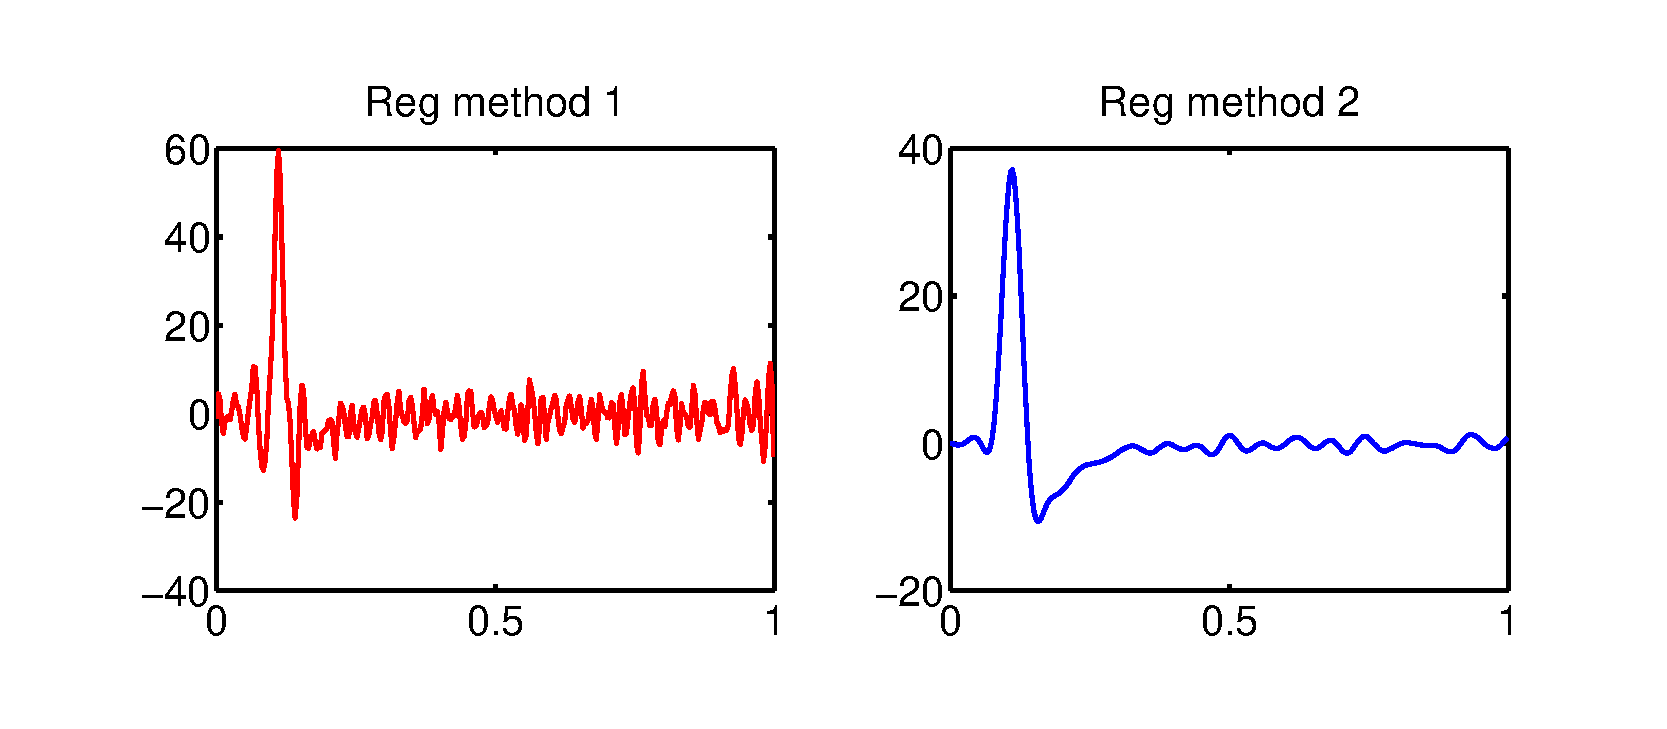
\includegraphics [width=\textwidth]{FilterEstimation_14.pdf}
\begin{par}
Reg. method 2 leads to a minimum in the value of \textit{S} at \textit{r} = 1, which means that the mean of the eigenvalues of \textit{C} is chosen. This seems natural, and produces nice-looking filters with little high-frequency noise on them. The gain, though, is off, but can be corrected post-hoc by scaling the filter:
\end{par} \vspace{1em}

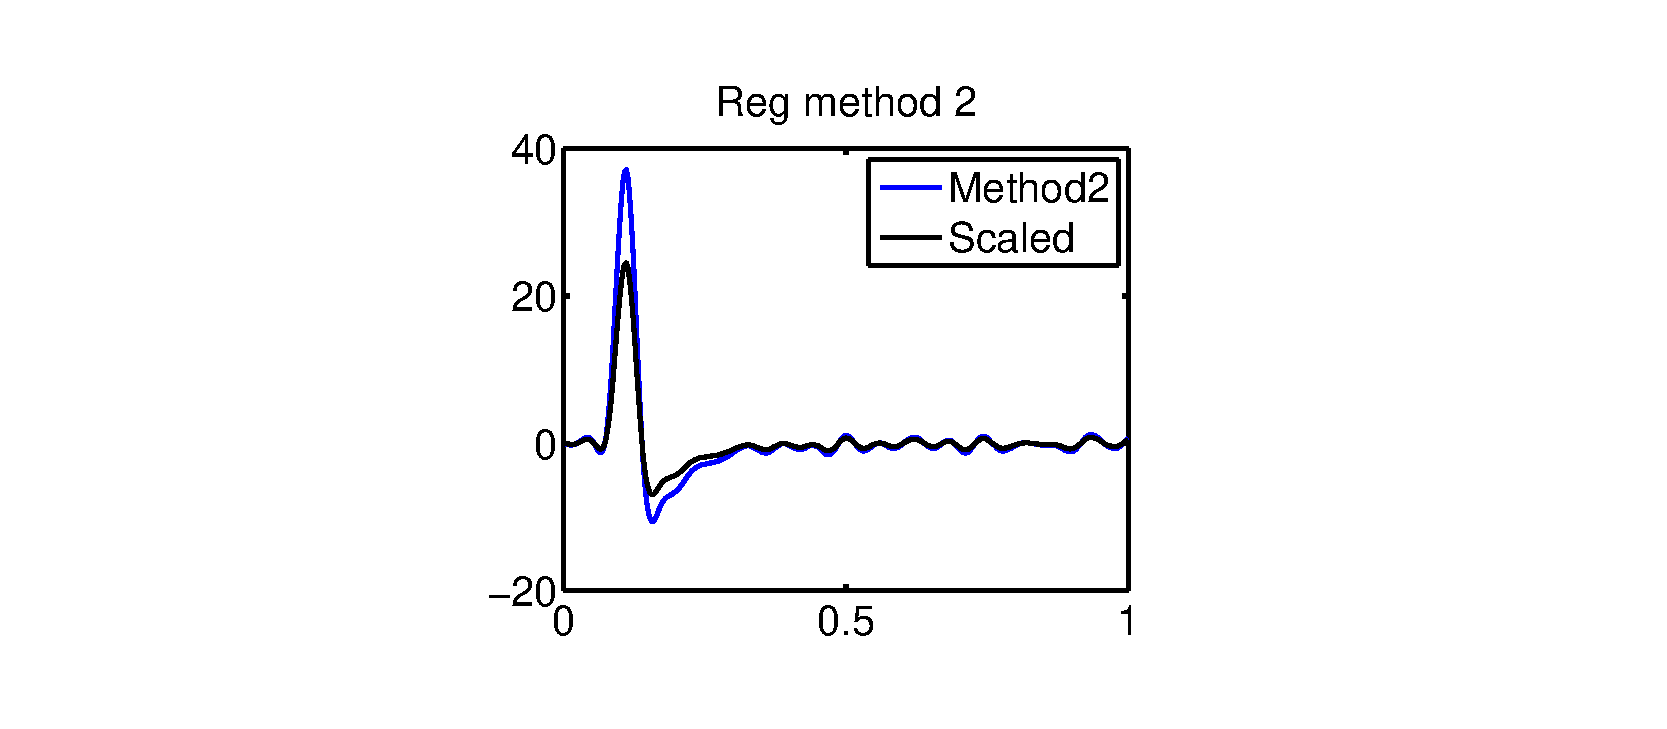
\includegraphics [width=\textwidth]{FilterEstimation_15.pdf}
\begin{par}
This filter now has gain of exactly 1. The prediction is pretty good:
\end{par} \vspace{1em}

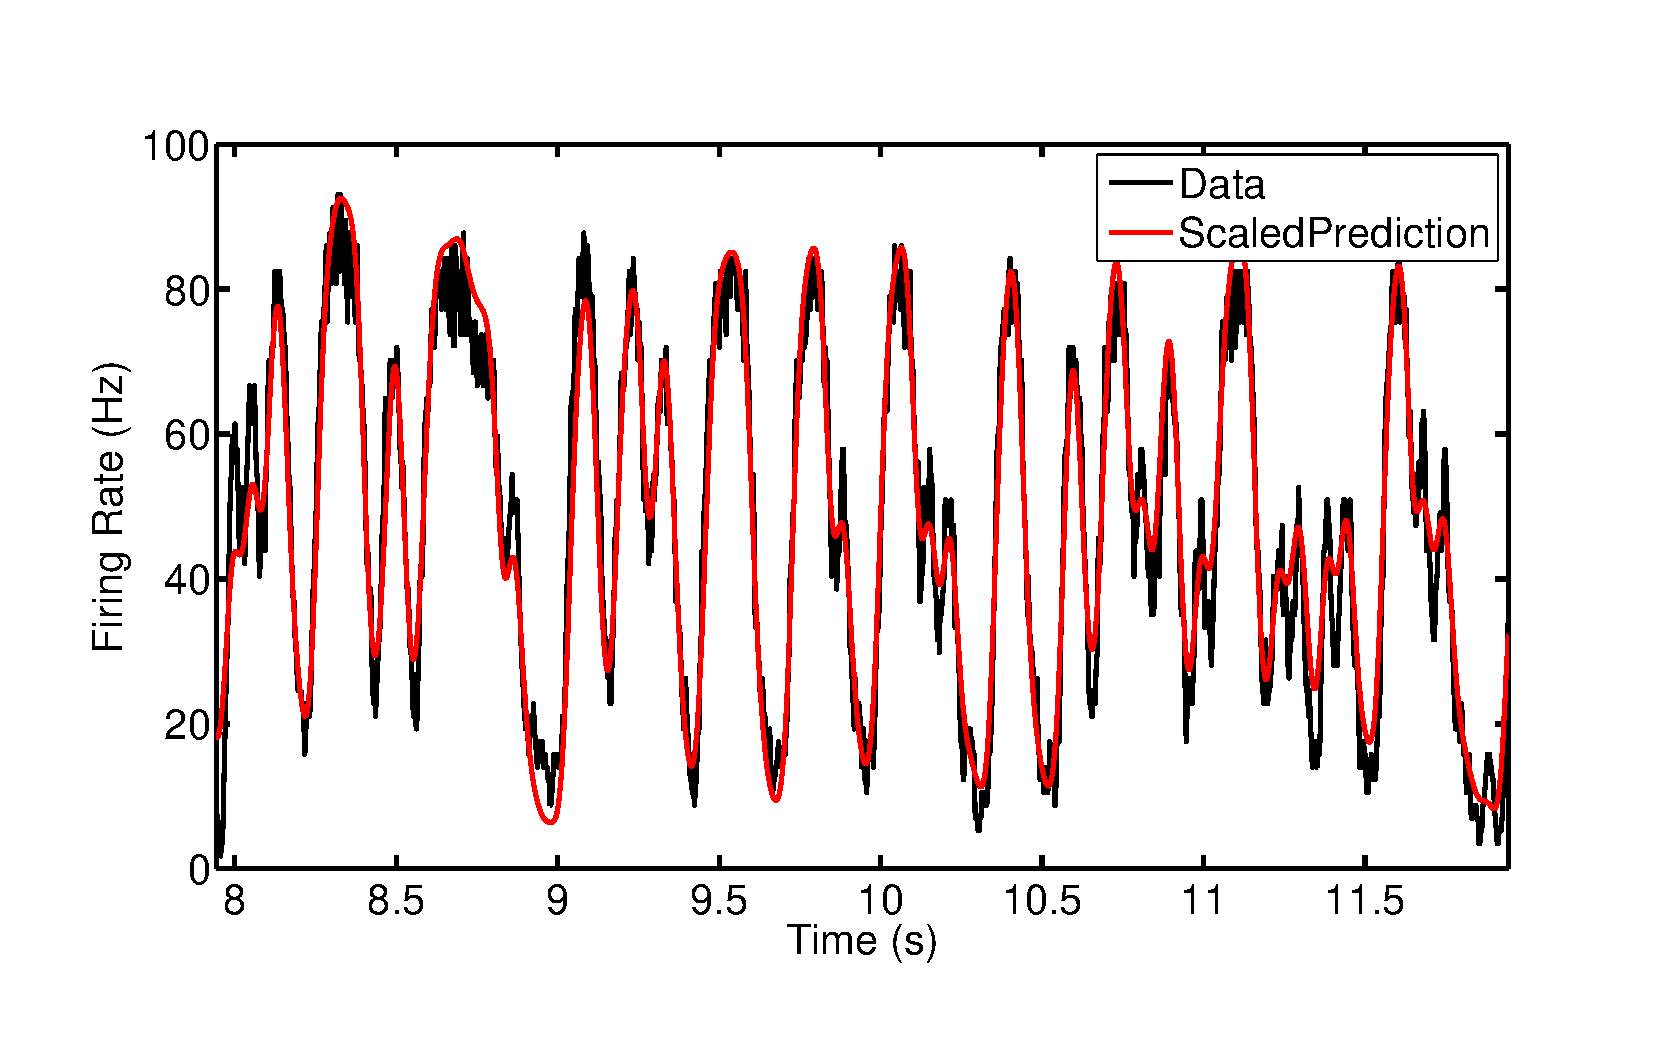
\includegraphics [width=\textwidth]{FilterEstimation_16.pdf}
\begin{par}
The r-square of this prediction is
\end{par} \vspace{1em}

        \color{lightgray} \begin{verbatim}    0.9279

\end{verbatim} \color{black}
    \begin{par}
and the best prediction from all the regularisation factors has a r-square of:
\end{par} \vspace{1em}

        \color{lightgray} \begin{verbatim}    0.9446

\end{verbatim} \color{black}
    


\end{document}
    
